\documentclass{article}

\usepackage{hyperref}
\usepackage{graphicx}
\usepackage{float}


\hypersetup{
    colorlinks=true,
    linkcolor=blue,
    filecolor=magenta,
    urlcolor=cyan,
}

\author{Kolobok team}
\title{Tire Text Extraction Research}
\date{July 2025}

\begin{document}
\maketitle

\section{Introduction}

One essential part of our project is a service for extracting information about a tire from an image. Performance of a standalone OCR model has proven to be insufficient and hard to improve. This problem arose in every of our previous approaches:

\begin{itemize}
    \item \textbf{Text detection + OCR} - we have tried to use vanilla OCR models, but their performance was too poor on tire images, as text styling and visibility varies across different examples. In addition, before we acquired a tire database, it was non-trivial how to interpret the output of OCR pipeline.
    \item \textbf{VLM as OCR} - we have tried to use VLM models as OCR, and got outstanding results for large and expensive models (\textbf{Gemini-2.5-Pro}, \textbf{GPT-4o}, \textbf{GPT-o3}), and much cheaper results for smaller and faster models (\textbf{Qwen-2.5-VL-32B-Instruct}). This limitation for smaller models can be explained by the fact that it was instructed not only to extract text, but also analyze it and return tire brand, model, and size, which introduced a lot of complexity.
\end{itemize}

To achieve better results without paying more, we needed to find a way to improve the performance of OCR pipeline.

\section{Dataset collection \& Manual annotation}

For experimental setup, we had to build an evaluation pipeline, so that we can easily test our changes and apply only the right ones.

\subsection{Dataset}

We collected a small, but diverse dataset of 42 images and manually annotated them with their \texttt{model\_id} and \texttt{brand\_id} from our database, as shown in Figure \ref{fig:dataset_examples}. Later, we will evaluate the performance of our pipeline on this dataset by comparing its predictions with the ground truth and evaluating the following metrics:

\begin{itemize}
    \item \textbf{Acc@1} - the fraction of correctly predicted \texttt{model\_id} and \texttt{brand\_id} pairs.
    \item \textbf{Acc@5} - the fraction of examples with at least one correct prediction in the top 5 predictions.
    \item \textbf{Average similarity} - average value of \texttt{Levenshtein ratio} between top-1 prediction and ground truth.
\end{itemize}

Initial metrics of our OCR pipeline can be seen in the table \ref{tab:initial_metrics}.

\begin{table}[h]
    \centering
    \begin{tabular}{|l|c|c|c|}
        \hline
        \textbf{Model} & \textbf{Acc@1} & \textbf{Acc@5} & \textbf{Avg Sim} \\
        \hline
        \textbf{Qwen-2.5-VL-32B} & 0.071 (3/42) & N/A & 0.7377 \\
        \hline
        \textbf{GPT-4o-mini} & 0.571 (24/42) & N/A & 0.8612 \\
        \hline
    \end{tabular}
    \caption{Initial metrics of our OCR pipeline}
    \label{tab:initial_metrics}
\end{table}

\begin{figure}[H]
    \centering
    \begin{tabular}{ccc}
        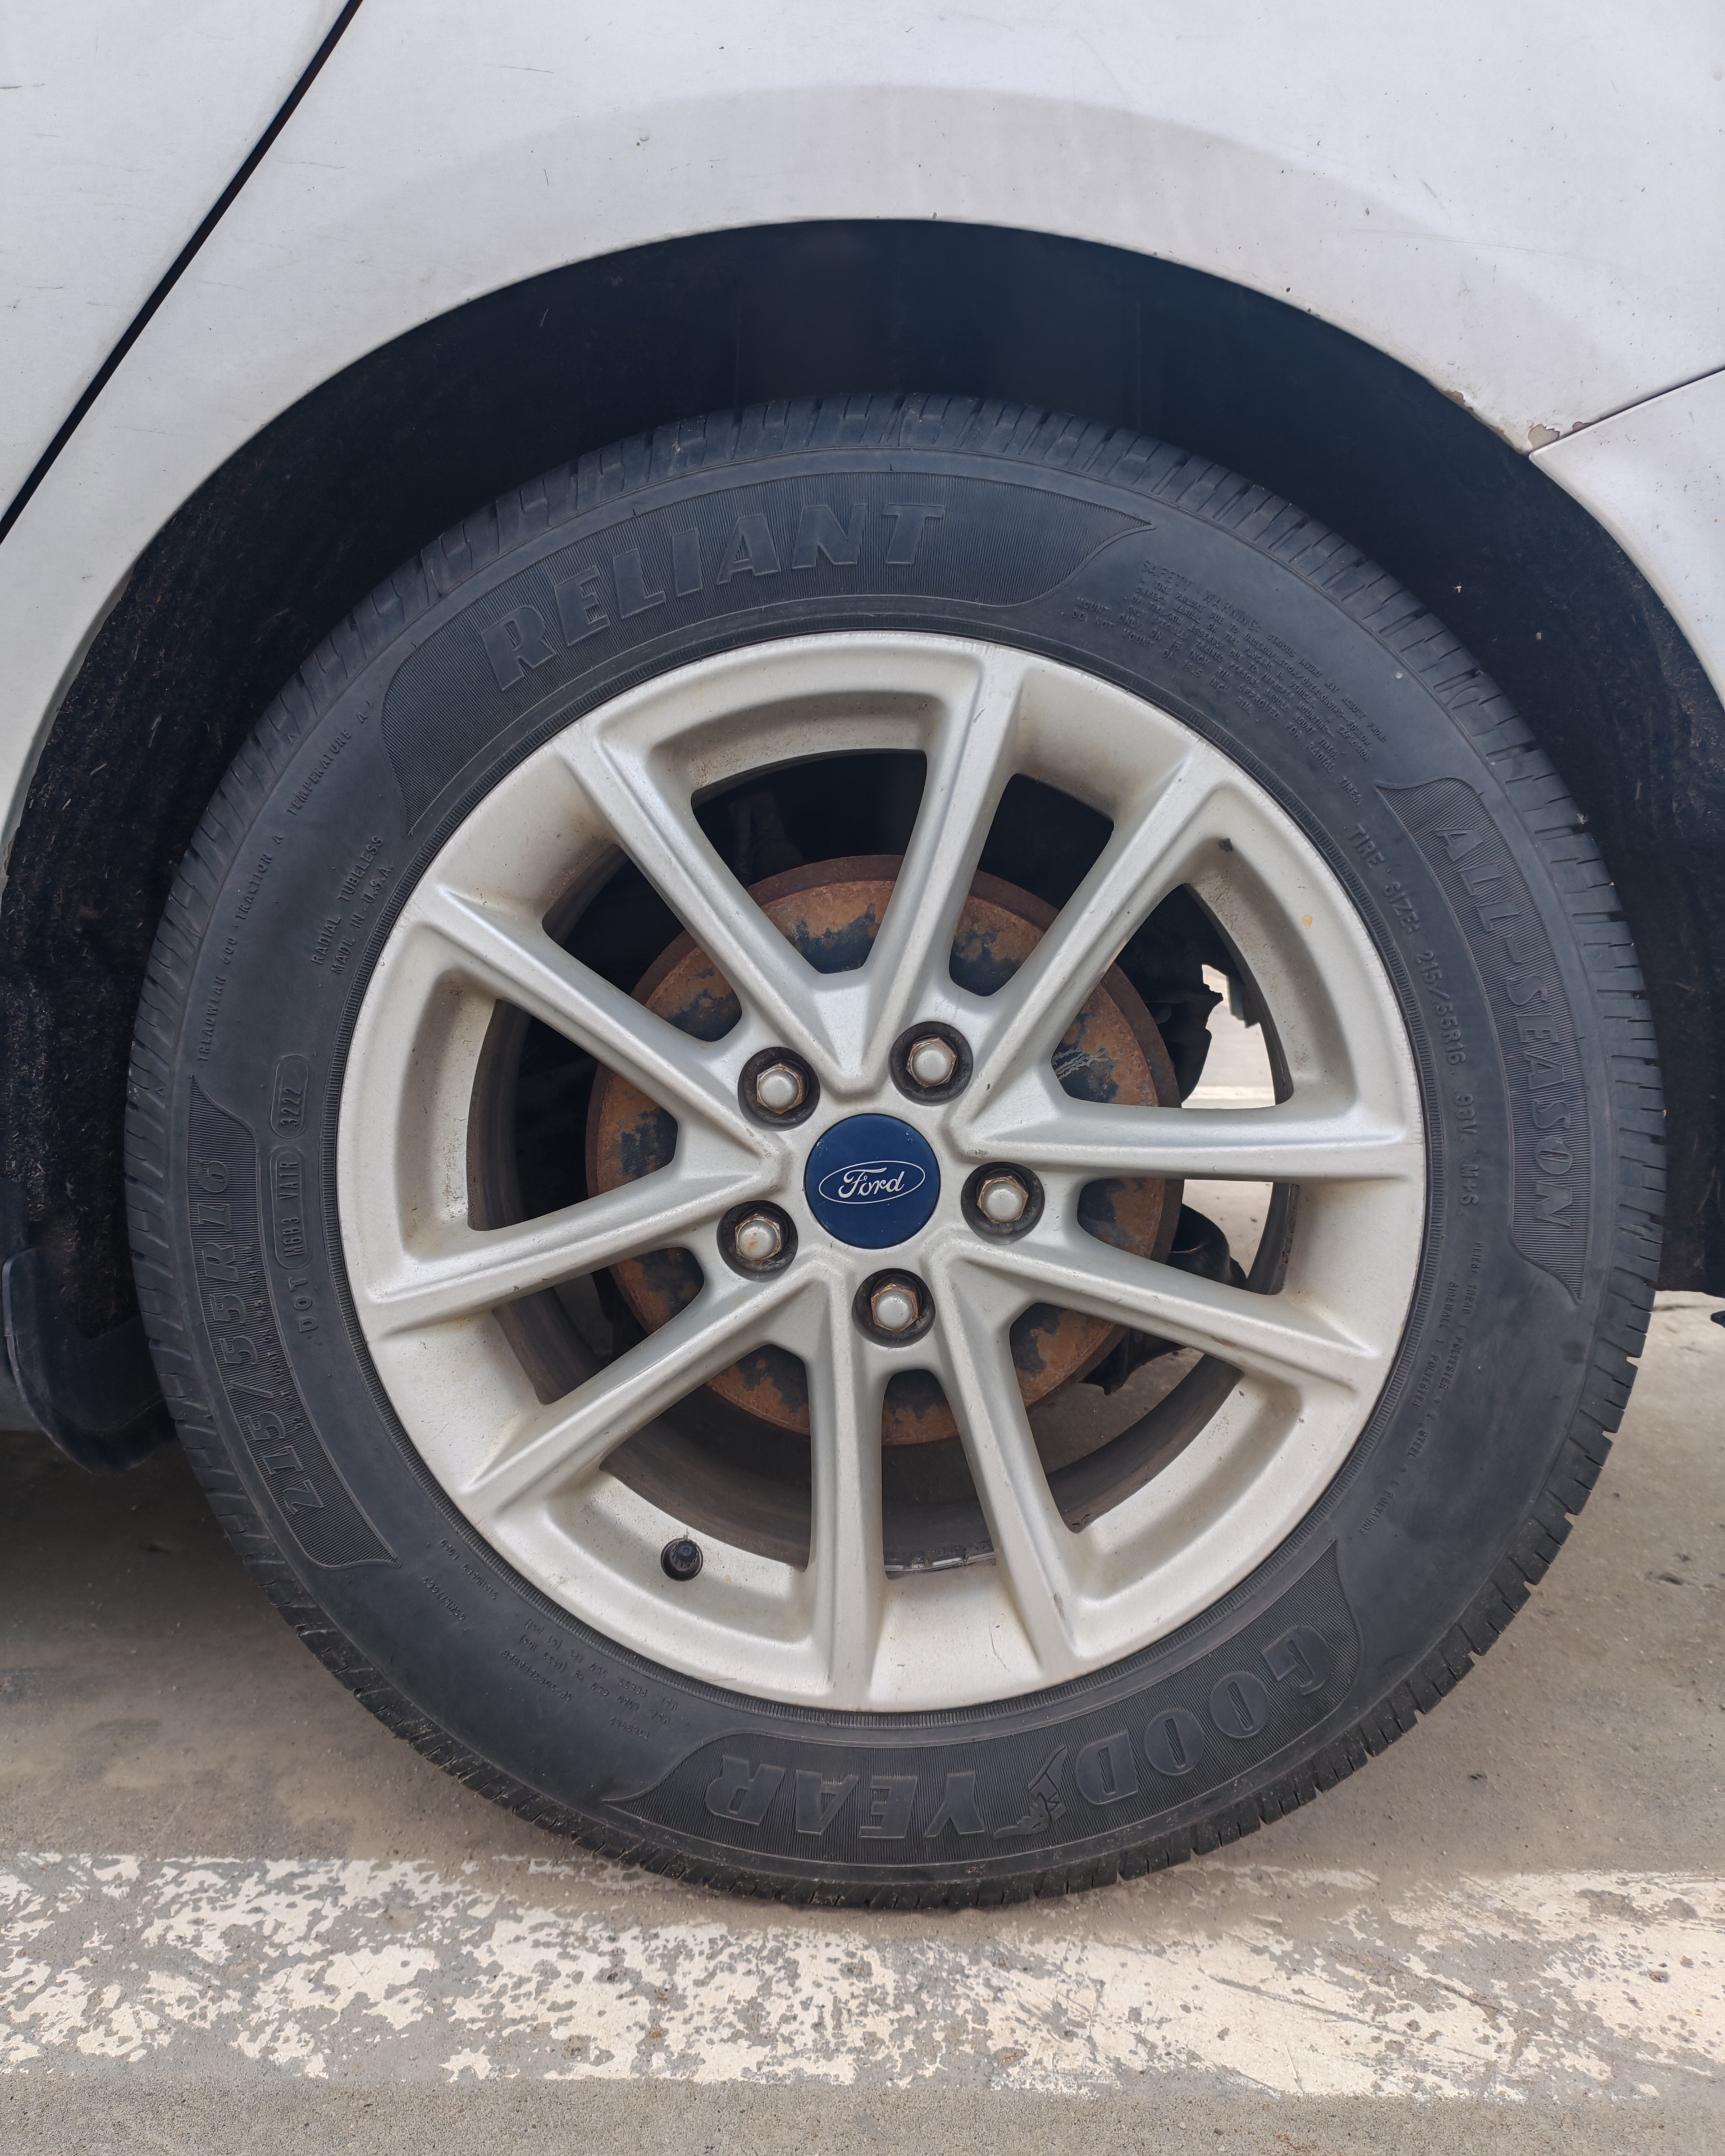
\includegraphics[width=0.27\textwidth]{assets/text_dataset/raw0.jpg} &
        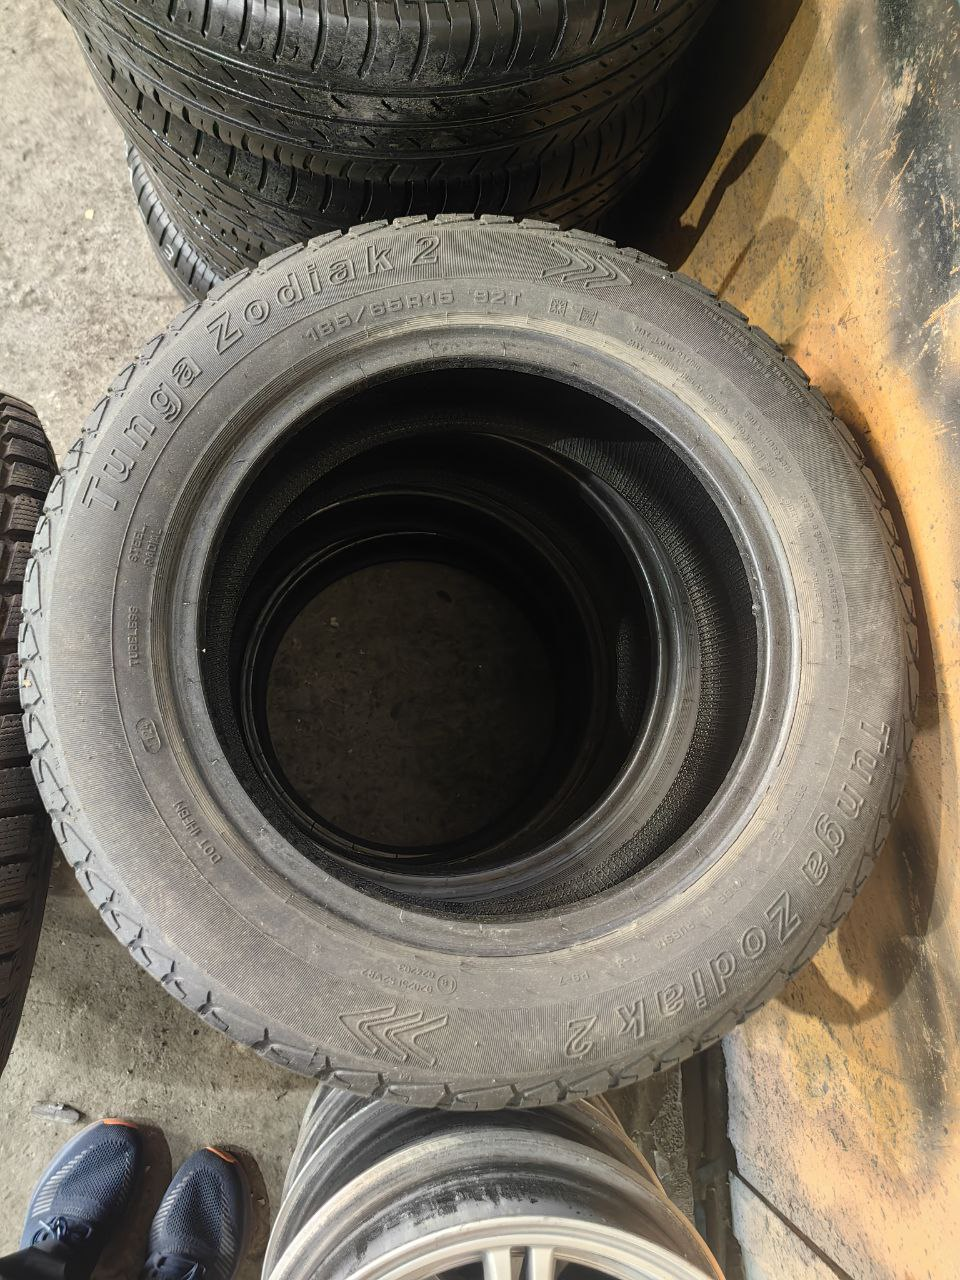
\includegraphics[width=0.27\textwidth]{assets/text_dataset/raw1.jpg} &
        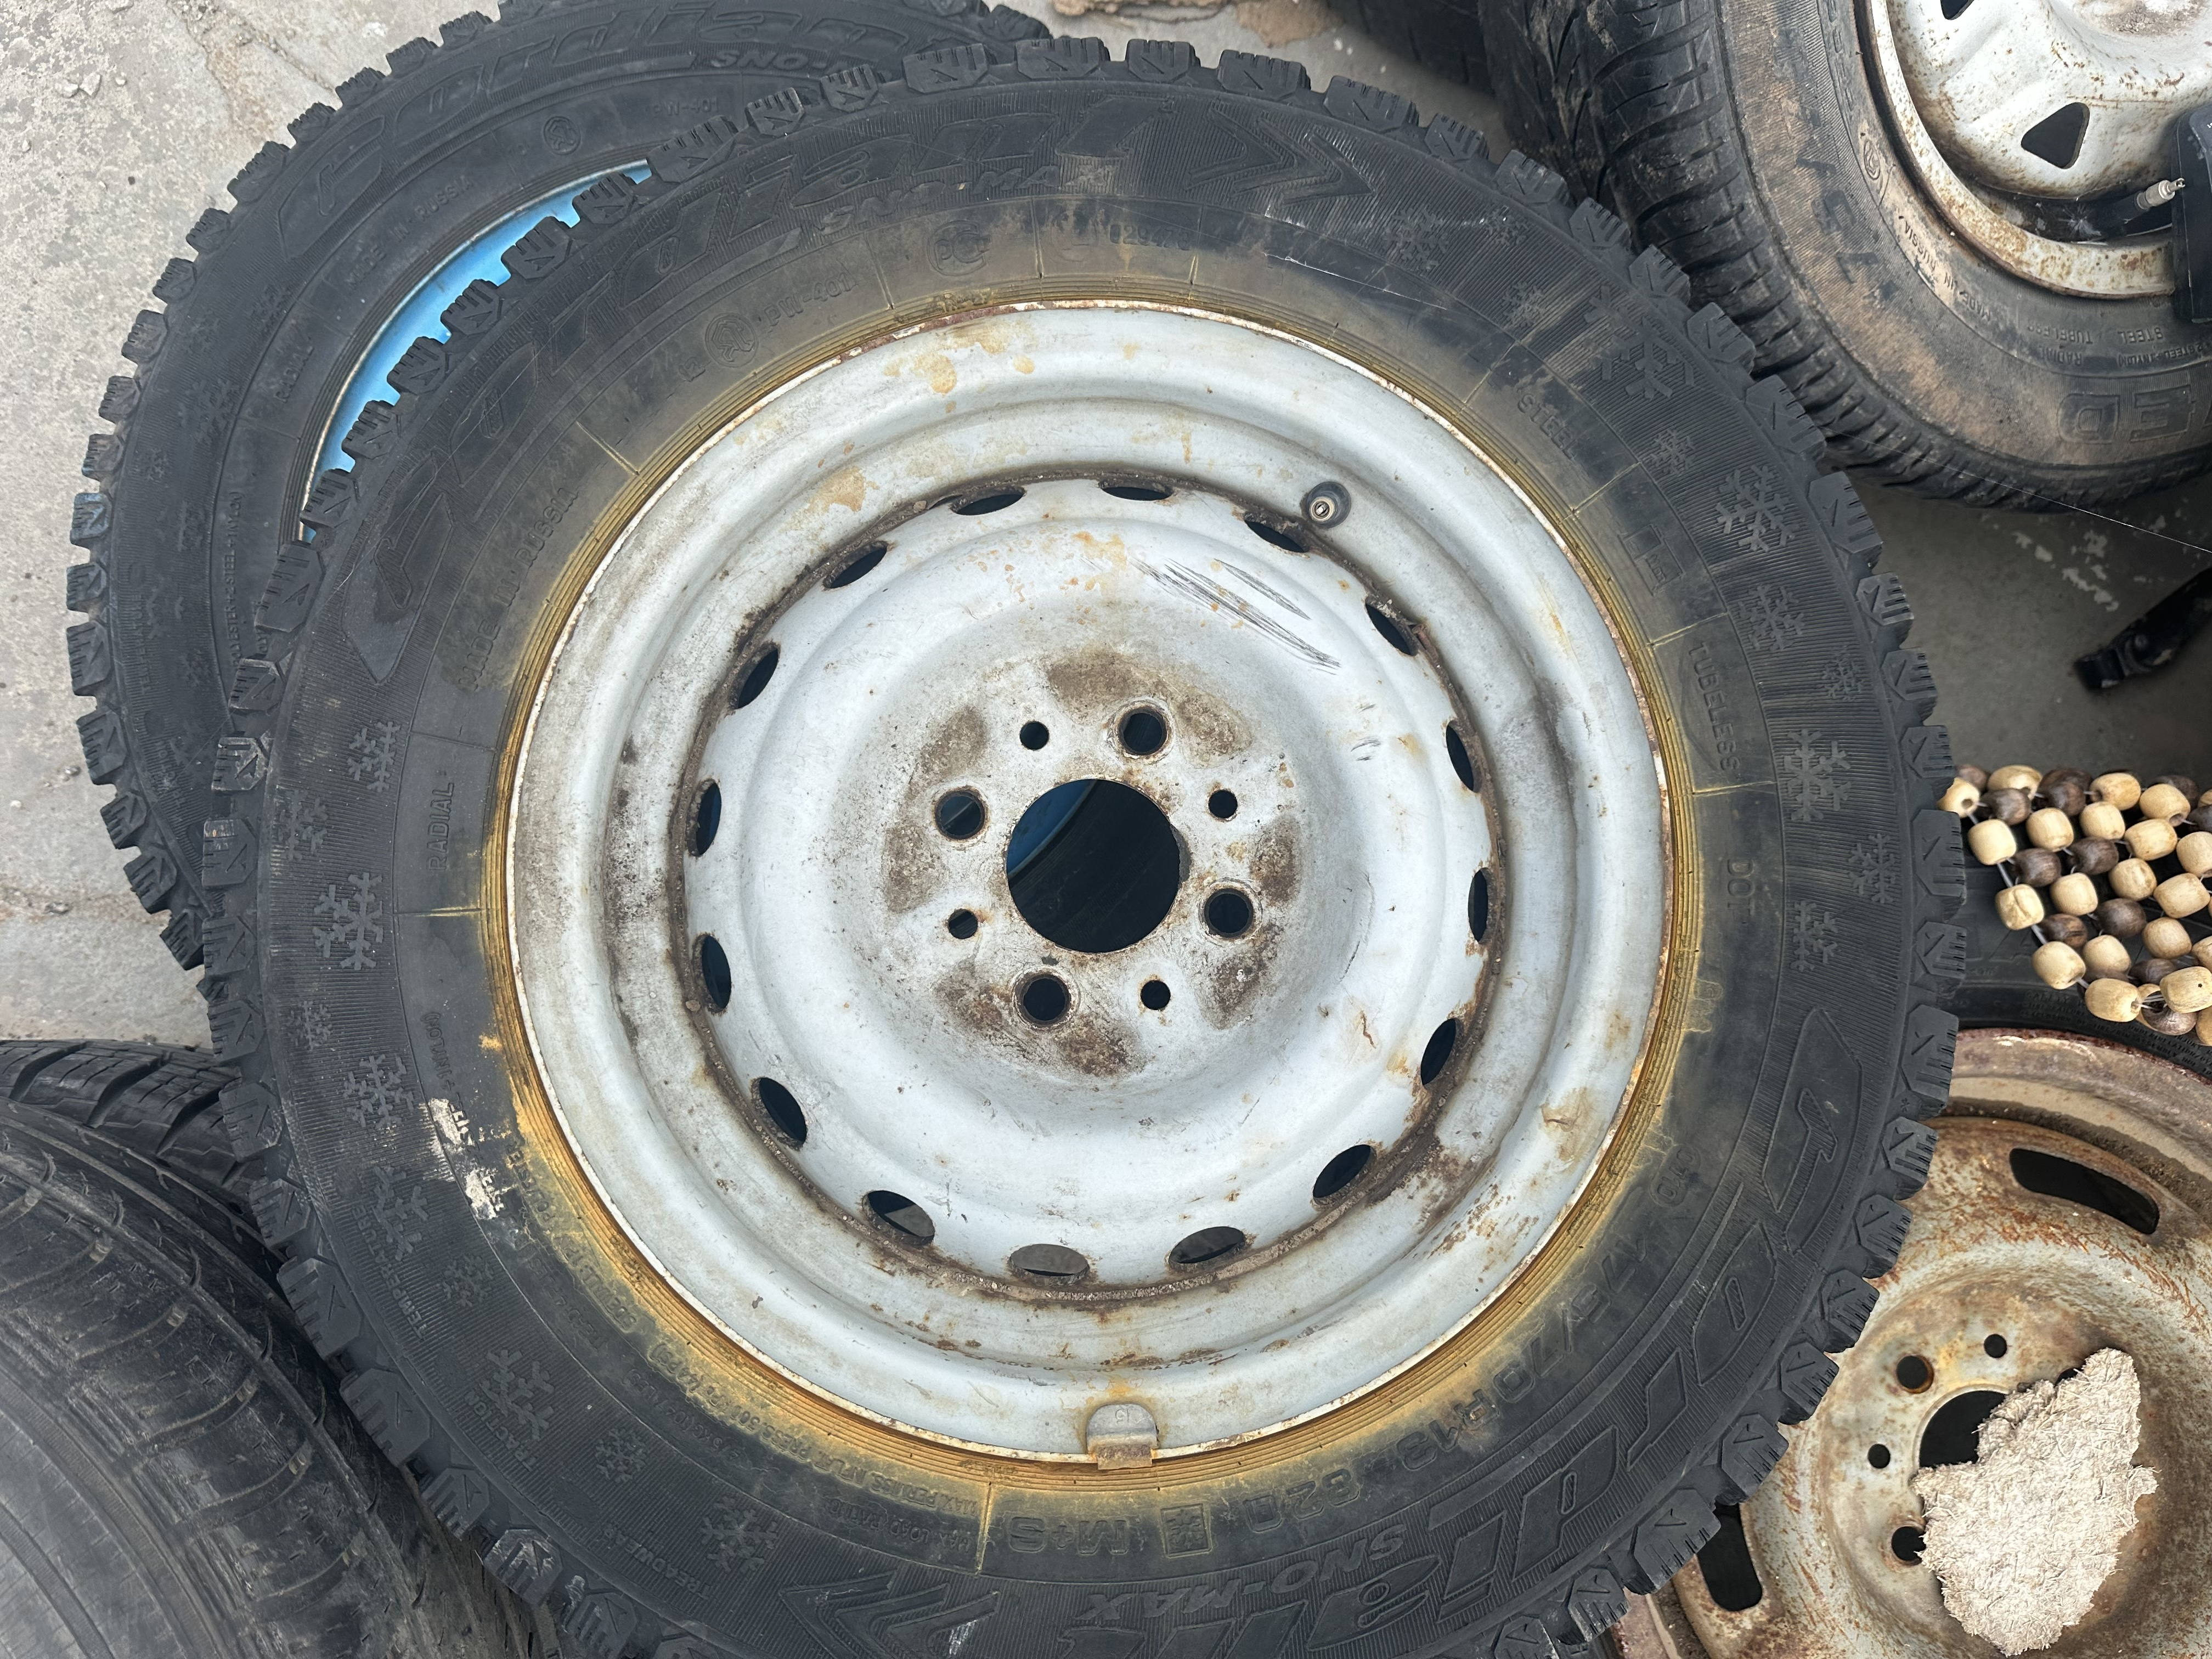
\includegraphics[width=0.27\textwidth]{assets/text_dataset/raw2.jpg}                                                                     \\
        \small Raw Image 1                                                  & \small Raw Image 2              & \small Raw Image 3              \\
        \small \texttt{model\_id: null}                                     & \small \texttt{model\_id: 3909} & \small \texttt{model\_id: 1625} \\
        \small \texttt{brand\_id: 14}                                       & \small \texttt{brand\_id: 40}   & \small \texttt{brand\_id: 10}   \\
    \end{tabular}
    \caption{Dataset examples showing raw tire images with their ground truth annotations. \texttt{null} means that this specific model or brand is not present in our database.}
    \label{fig:dataset_examples}
\end{figure}

\section{Enhancement plan}

In our pipeline, there are currently three components that require improvement:

\begin{itemize}
    \item \textbf{Tire unwrapping} - consists of a segmentation model and a perspective transformation. Previously, we used a simple pre-trained model, which did not have very high performance: \href{https://universe.roboflow.com/my-workspace-xwpro/tire-segmentation-eqoeu}{Roboflow model}. The segmentation results were passed to a perspective transformation pipeline, which was implemented using \href{https://docs.opencv.org/4.x/da/d54/group__imgproc__transform.html}{OpenCV} geometric image transformations. Results of this pipeline are shown in Figure \ref{fig:unwrapped_examples}.
    \item \textbf{OCR} - a VLM model, which was prompted to extract all required fields from the unwrapped tire image.
    \item \textbf{Index (new)} - a lookup table, which is used to postprocess the OCR result by performing fuzzy matching with existing tire models and brands.
\end{itemize}

\begin{figure}[H]
    \centering
    \begin{tabular}{ccc}
        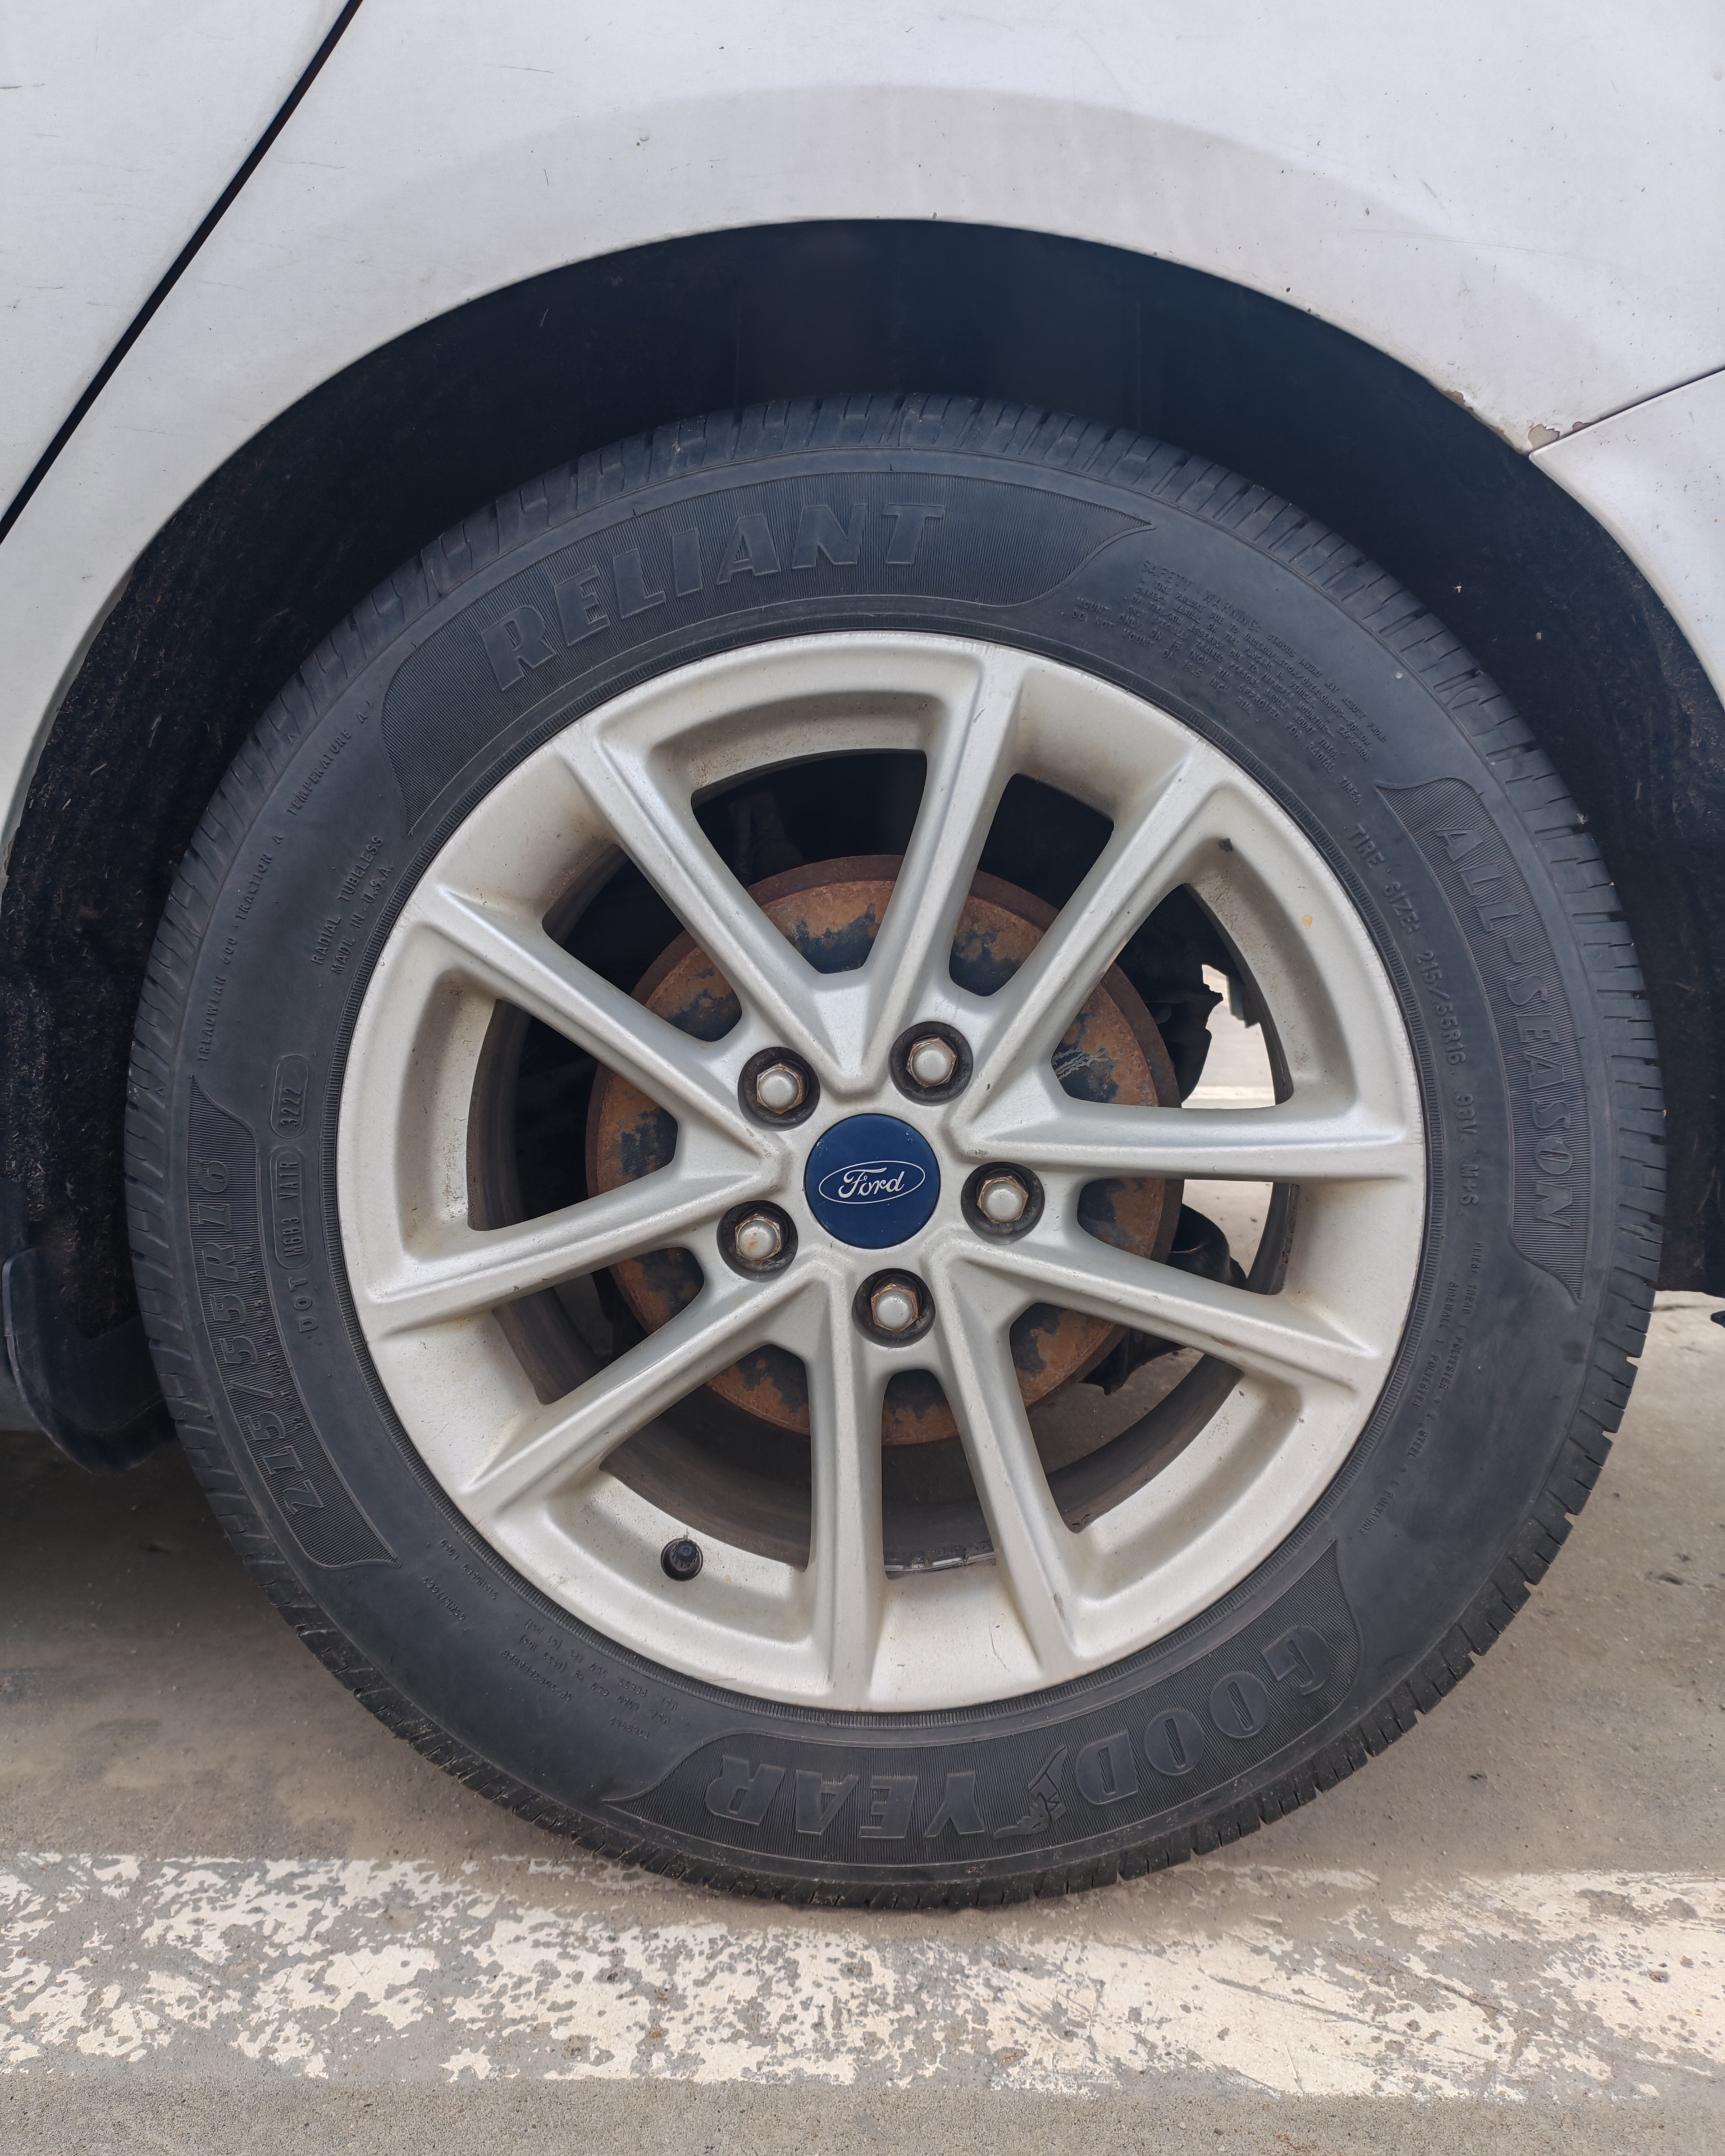
\includegraphics[width=0.27\textwidth]{assets/text_dataset/raw0.jpg}       &
        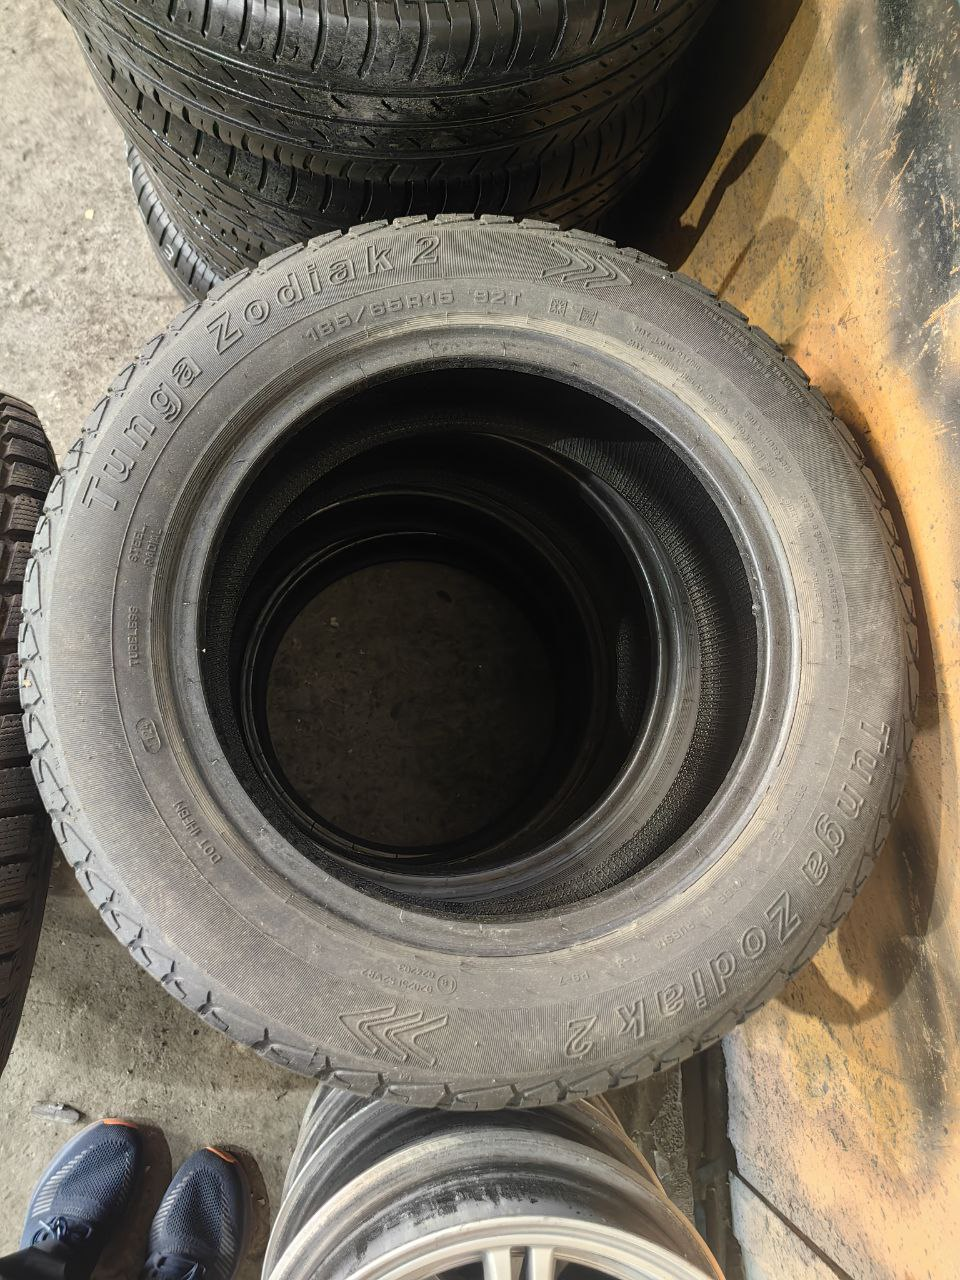
\includegraphics[width=0.27\textwidth]{assets/text_dataset/raw1.jpg}       &
        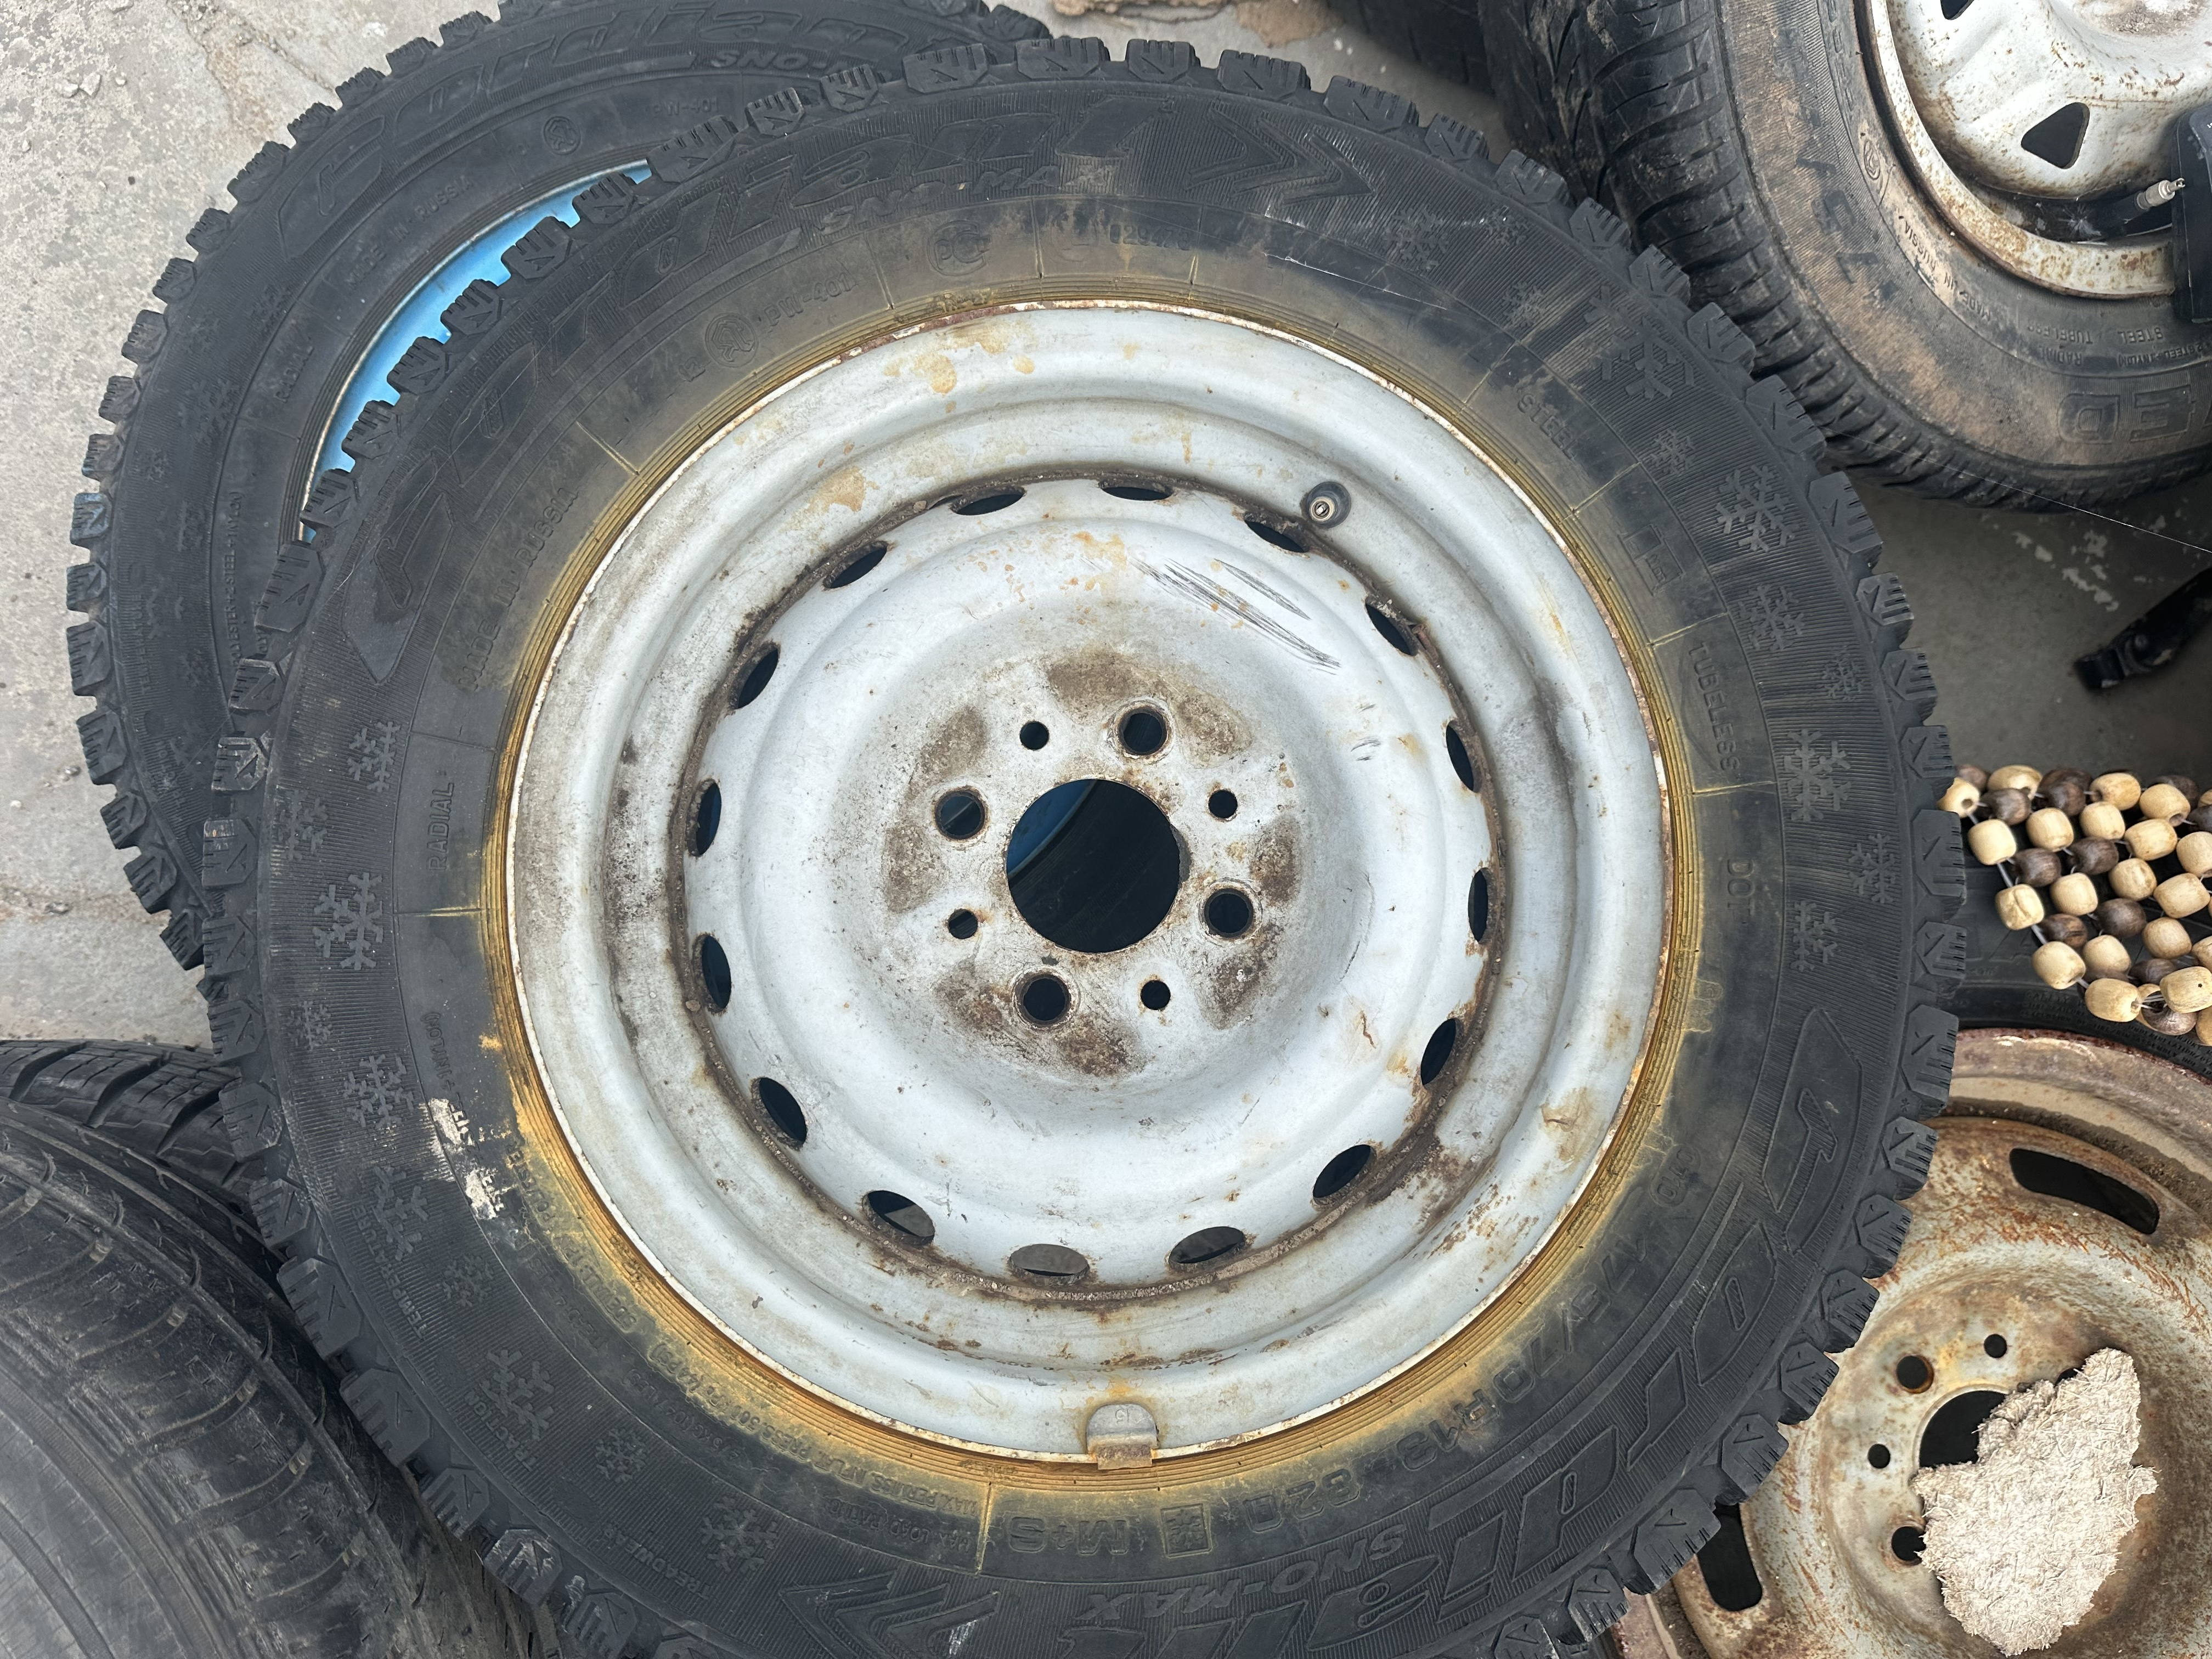
\includegraphics[width=0.27\textwidth]{assets/text_dataset/raw2.jpg}                                                             \\
        \includegraphics[width=0.27\textwidth]{assets/text_dataset/unwrapped0.png} &
        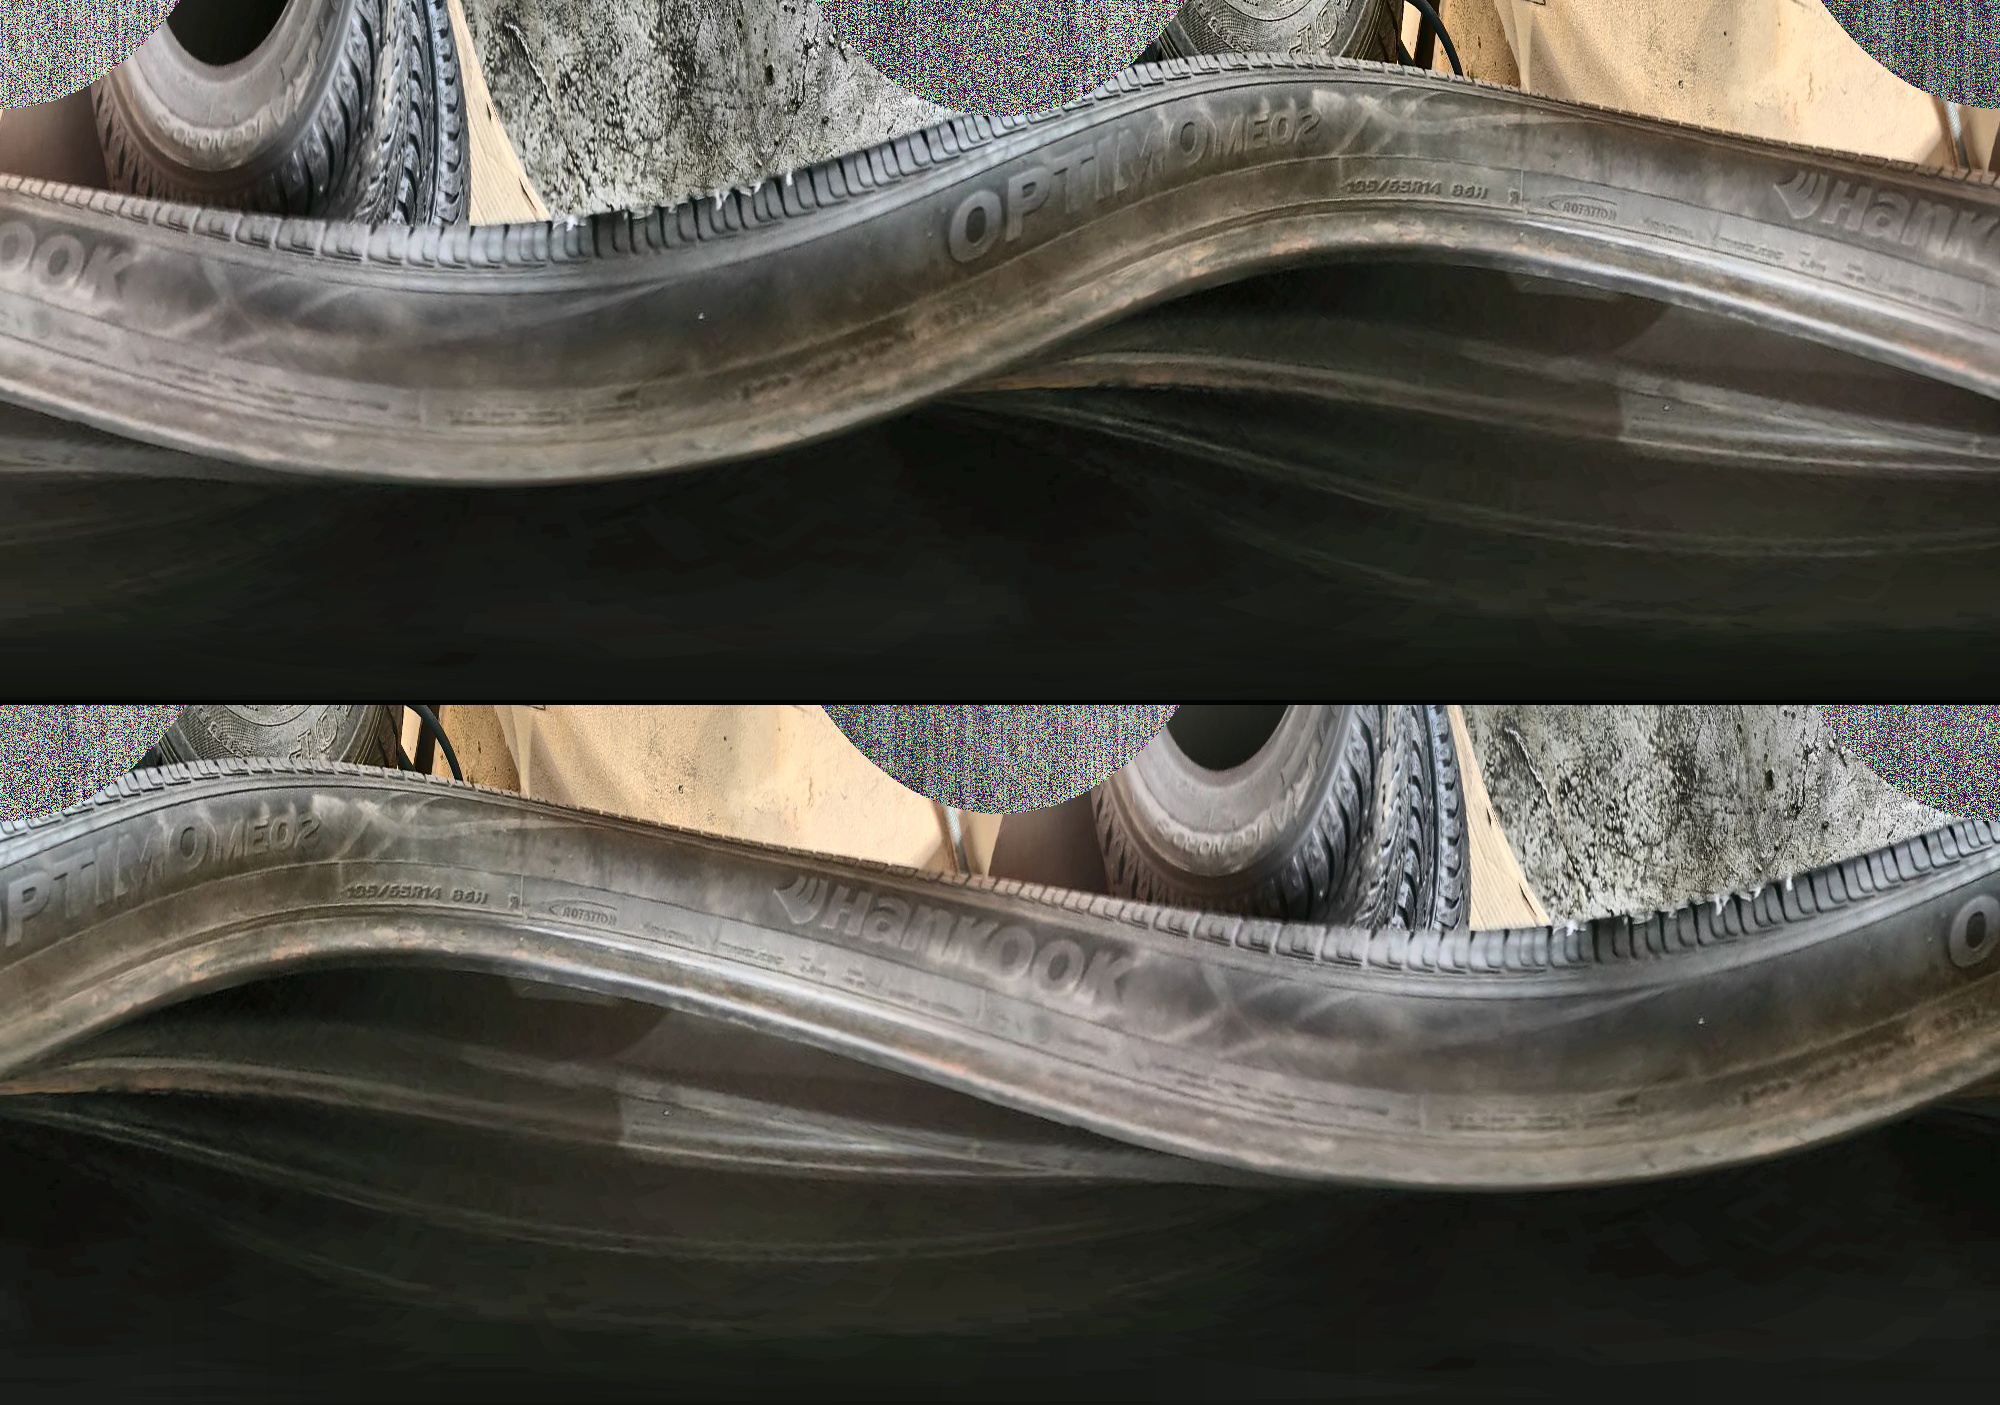
\includegraphics[width=0.27\textwidth]{assets/text_dataset/unwrapped1.png} &
        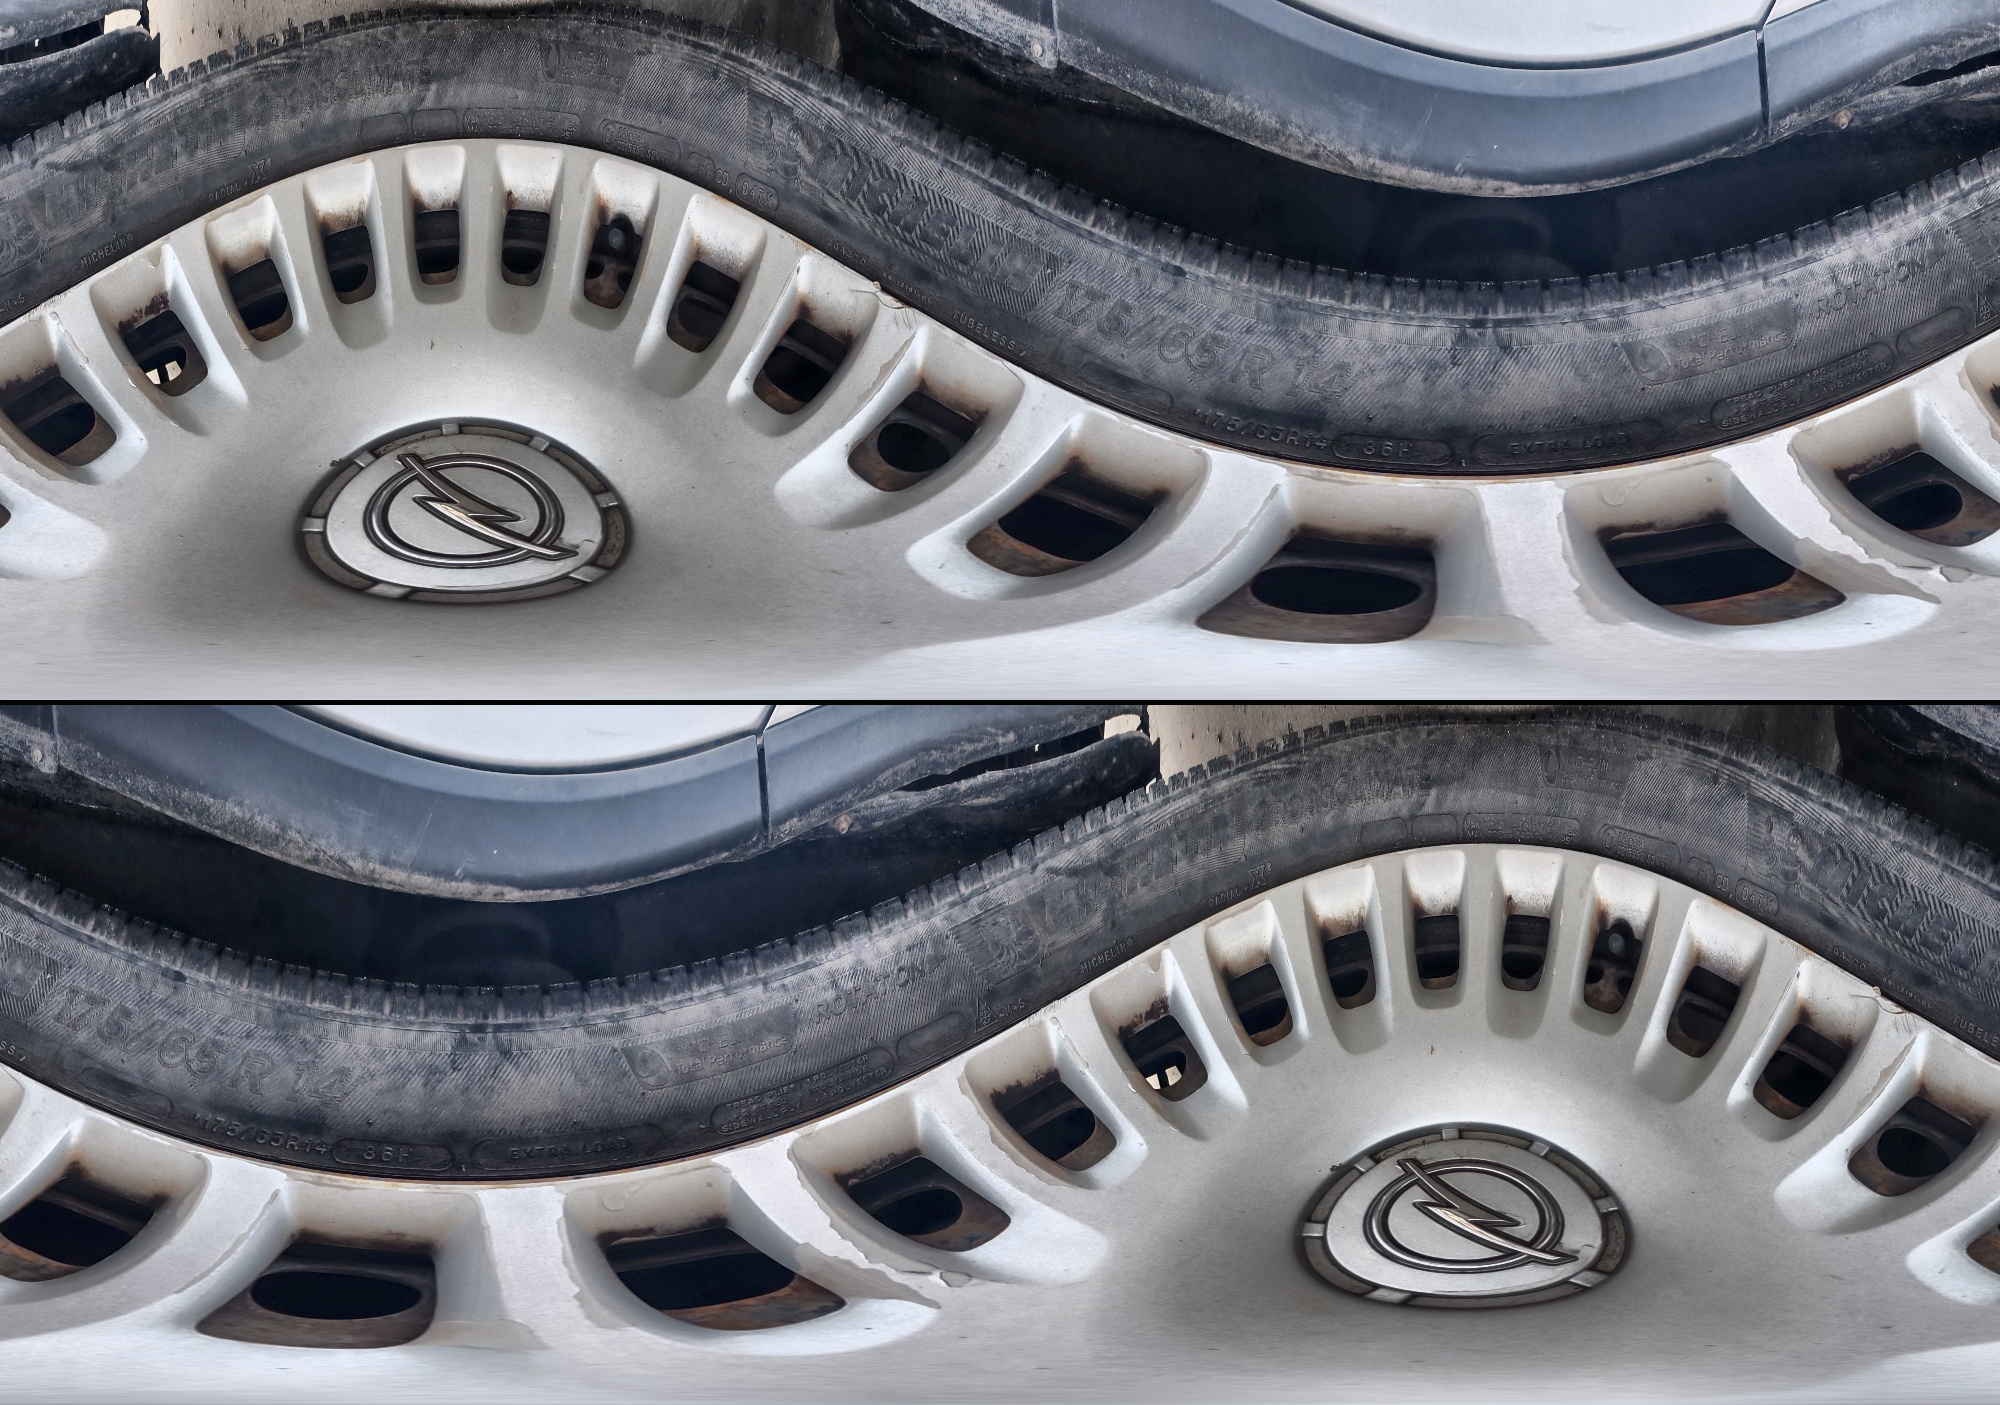
\includegraphics[width=0.27\textwidth]{assets/text_dataset/unwrapped2.png}                                                       \\
        \small Unwrapped Image 1                                                  & \small Unwrapped Image 2 & \small Unwrapped Image 3 \\
    \end{tabular}
    \label{fig:unwrapped_examples}
\end{figure}

\section{Tire Unwrapping improvement}

\subsection{Model}
The model we used for segmenting tires was light-weight, but not very accurate. In order to improve the performance, we trained our own model of \texttt{SegFormer} architecture on this \href{https://universe.roboflow.com/segmentation-k0zny/tyre-wpkj0}{Roboflow dataset} with 600 images. To improve the capability of the model to segment only front-view wheel of the image, we augmented the dataset and added custom background images filled with tires, as shown in Figure \ref{fig:seg_augmentation}.

\begin{figure}[H]
    \centering
    \begin{tabular}{cc}
        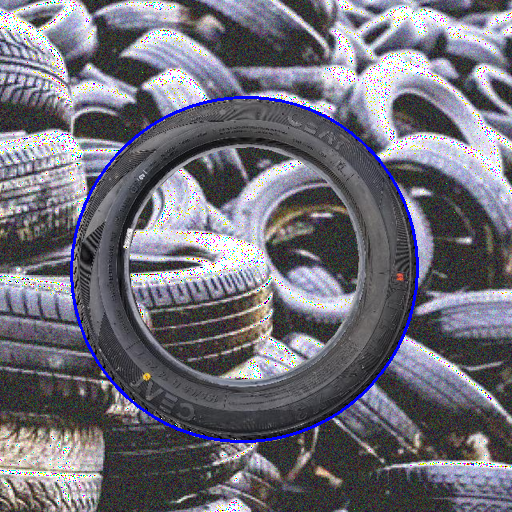
\includegraphics[width=0.45\textwidth]{assets/seg_aug_dataset/aug0.png} &
        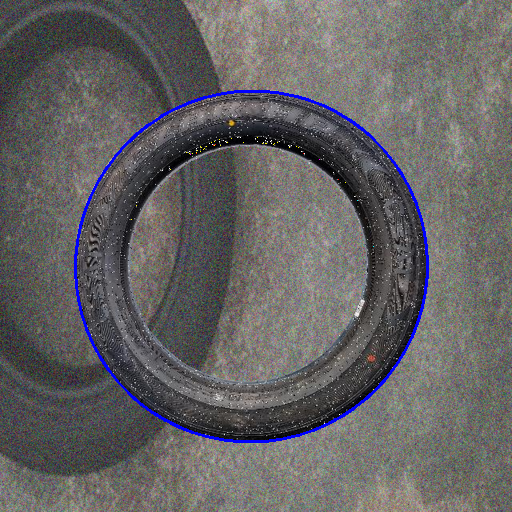
\includegraphics[width=0.45\textwidth]{assets/seg_aug_dataset/aug1.png}                            \\
        \small Augmented Image 1                                                & \small Augmented Image 2 \\[0.5em]

        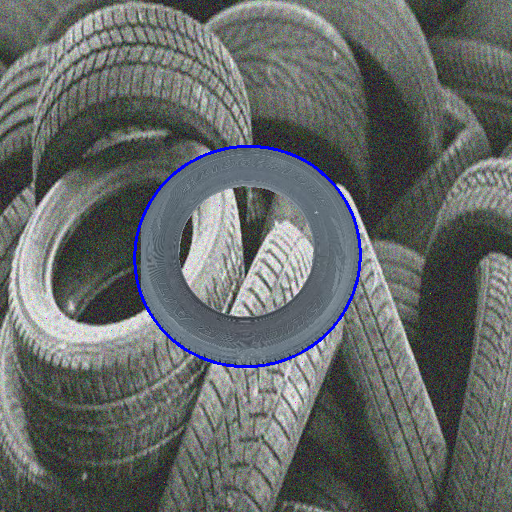
\includegraphics[width=0.45\textwidth]{assets/seg_aug_dataset/aug2.png} &
        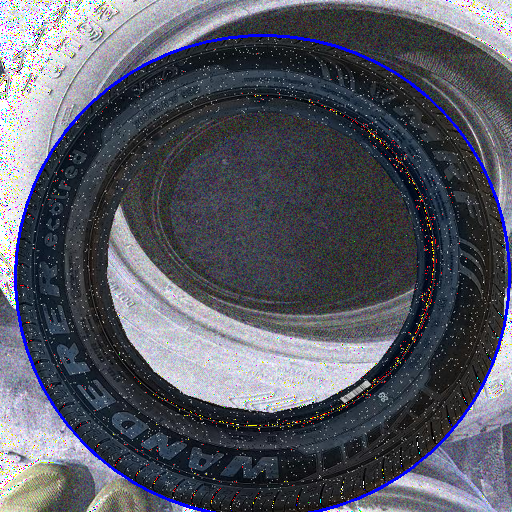
\includegraphics[width=0.45\textwidth]{assets/seg_aug_dataset/aug3.png}                            \\
        \small Augmented Image 3                                                & \small Augmented Image 4 \\
    \end{tabular}
    \caption{Examples of dataset augmentation for tire segmentation training. Custom background images with multiple tires help improve the model's ability to segment front-view wheels specifically (highlighted in blue).}
    \label{fig:seg_augmentation}
\end{figure}

\subsection{Unwrapping \& Postprocessing}
To get more perceptually prominent textual information on resulting images, we introduced a series of minor enhancements to the unwrapping pipeline:

\begin{itemize}
    \item \textbf{Constant shape unwrapping} - to avoid possible distortions, we scale polar unwrapping to a constant shape ($2000 \times 700$ pixels).
    \item \textbf{Fitting an Ellipse to the segmentation} - to improve stability of our postprocessing pipeline, we fit an ellipse to the segmentation mask and use it instead of mask for computing required perspective transforms.
    \item \textbf{Conditional translation} - to properly unwrap the tires which have significant rotation with respect to the camera view, we conditionally translate the image (ellipse to circle), if its foci have too large distance.
    \item \textbf{CLAHE improvement} - we apply CLAHE contrast enhancement to the image to make text more prominent. To make it more robust, we apply it only to \textbf{Luminance} component of the image, instead of grayscale.
\end{itemize}

\section{Relaxation of OCR bottleneck}

Since we got a database with fuzzy matching capabilities, we can now relax the task for VLM model from extracting all required information to extracting only text, which is much easier task and can be done by \textbf{Qwen-2.5-VL-32B-Instruct} model. The model is tasked to extract all textual entries from the unwrapped tire and return them as a list of strings.

\section{Index integration}

Since last sprint, we have acquired an access to a database containing approximately 10000 tire model entries. This database is hosted as \textbf{MySQL} database, which introduces some challenges for our fuzzy matching pipeline.

\subsection{SQL UDF}

Since \textbf{MySQL} lacks support for community extensions (like \texttt{fuzzystrmatch} for \textbf{PostgreSQL}), we have to implement our own fuzzy matching function, which computes \texttt{Levenshtein ratio} between two strings. This approach proved to be extremely slow, as \textbf{MySQL} is not optimized for such operations (approximately 10 seconds for 50000 function calls).

\subsection{Polars}

Since the database is not expected to grow significantly, we have taken a different approach. We download the entire table into the memory and utilize lazy evaluation feature of \textbf{Polars} library to perform faster fuzzy matching. This approach significantly optimized the performance of our fuzzy matching algorithm, allowing us to perform full search of OCR result (5-10 strings on average) against the database (10000 entries) in approximately 0.2 seconds.

\section{Results}

Combining all the changes, we observe the following results on our dataset:

\begin{table}[H]
    \centering
    \begin{tabular}{|l|c|c|c|}
        \hline
        \textbf{Model} & \textbf{Acc@1} & \textbf{Acc@5} & \textbf{Avg Sim} \\
        \hline
        \textbf{Qwen-2.5-VL-32B} & 0.810 (34/42) & 0.905 (38/42) & 0.9560 \\
        \hline
    \end{tabular}
\end{table}

\end{document}